\documentclass{scrreprt}

\usepackage{graphicx}
\usepackage{tikz}
\usepackage{amstext}
\usepackage{amsfonts}
\usepackage{tabularx}
\usepackage{multirow}
\usepackage{amssymb}
\usepackage{textcomp}
\usepackage[left=2.5cm, right=2.5cm, top=2cm, bottom=2cm]{geometry}
\newcommand\tab[1][1cm]{\hspace*{#1}}

\usepackage{listings}
\usepackage{color}

\definecolor{dkgreen}{rgb}{0,0.6,0}
\definecolor{gray}{rgb}{0.5,0.5,0.5}
\definecolor{mauve}{rgb}{0.58,0,0.82}

\lstset{frame=tb,
  language=Java,
  aboveskip=3mm,
  belowskip=3mm,
  showstringspaces=false,
  columns=flexible,
  basicstyle={\small\ttfamily},
  numbers=none,
  numberstyle=\tiny\color{gray},
  keywordstyle=\color{blue},
  commentstyle=\color{dkgreen},
  stringstyle=\color{mauve},
  breaklines=true,
  breakatwhitespace=true,
  tabsize=3
}


\title{\textbf{Algorithmen und Datenstrukturen}}
\author{}
\begin{document}
\pagenumbering{gobble}
\maketitle
\pagebreak
\renewcommand{\contentsname}{Inhaltsverzeichnis}
%\renewcommand{\cftdot}{}
\setcounter{tocdepth}{1}
\tableofcontents
\pagebreak
%\pagenumbering{arabic}
\chapter{Mathematische Grundlagen}
\section{Reihen}
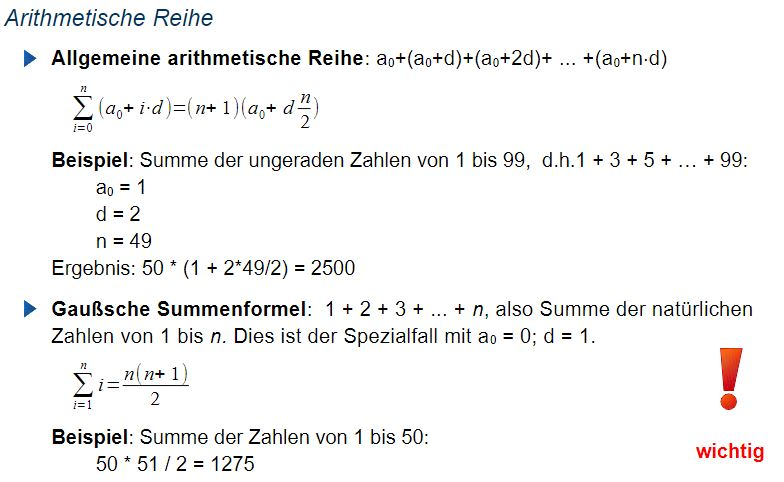
\includegraphics[width=0.65\textwidth]{graphics/reihen-arithmetisch}
\section{Potenzen und Logarithmen}
Der Logarithmus ist die Inverse der Potenzfunktion. $\log_a(x) = y \quad \Longleftrightarrow  \quad a^y = x$
\\\textbf{spezielle Logarithmen:}
\\$ld(x)=log_2(x)$, $lg(x)=log_10(x)$, $ln(x)=log_e(x)$
\section{Notationskonventionen}
$\lceil x \rceil$ zur nächsten ganzen Zahl aufrunden
\\$\lfloor x \rfloor$ zur nächsten ganzen Zahl abrunden
\\$[a .. b] = {x \arrowvert a \leq x \wedge x \leq b}$ mit Intervallgrenzen
\\$]a .. b[ = {x \arrowvert a < x \wedge x < b}$ ohne Intervallgrenzen
\\$arr[i .. k]$ Teilfolge der Elemente von $arr[i]$ bis $arr[k]$
\section{Grundbegriffe der Graphentheorie}
Graphen bestehen aus einer Menge von Knoten und Kanten, die diese verbinden.
\\Ein Graph ist gerichtet, wenn die Kanten eine Richtung haben.
\\Für einen Knoten v eines gerichteten Graphen $G=(V,E)$ ist der Eingangsgrad $indeg(v)$ die Anzahl der Kanten,
die in v enden, und der Ausgangsgrad $outdeg(v)$ die Anzahl der Kanten, die von v ausgehen.
\\Ein Zyklus ist ein Weg der bei einem Knoten startet und endet.
\\Ein gerichteter Graph ist zusammenhängend, wenn es einen Weg zwischen jedem Knotenpaar gibt.
\\Ein Baum hat einen Knoten als Wurzel, jeder Knoten hat genau einen Vorgänger und ist zusammenhängend.
\\Ein Knoten ohne Kinder heißt Blatt. Ein leerer Baum hat die Höhe 0.
Ein Binärbaum ist ein Baum, dessen Knoten maximal zwei Kinder haben.
\\Traversierungen: Preorder (WLR), Inorder (LWR), Postorder (LRW)
\chapter{Rekursive Algorithmen}
\section{Prinzip der Rekursion}
Ein rekursiver Algorithmus besteht aus einem Basisfall und einem rekursiven Aufruf.
\\Der rekursive Aufruf muss immer kleiner werden, damit die Rekursion endet.
\\Die Rekursion kann durch eine Schleife ersetzt werden.
\begin{lstlisting}
  public static double sum_v2(double[] arr) {
  return sum_v2(arr, 0, arr.length-1);
  }
/** Berechnet Summe der Werte von arr[firstIndex..lastIndex] */
  private static double sum_v2(double[] arr, int firstIndex,int lastIndex) {
  if (firstIndex == lastIndex) {
    // zu summierender Bereich besteht nur aus einem Element
    return arr[firstIndex];
  }
  else {
    int mid = (firstIndex + lastIndex) / 2;
    return sum_v2(arr, firstIndex, mid) + sum_v2(arr, mid+1, lastIndex);
  }}
  \end{lstlisting}
\section{Korrektheit rekursiver Algorithmen}
Ein Beweisverfahren ist die Berechnungsinduktion.
\\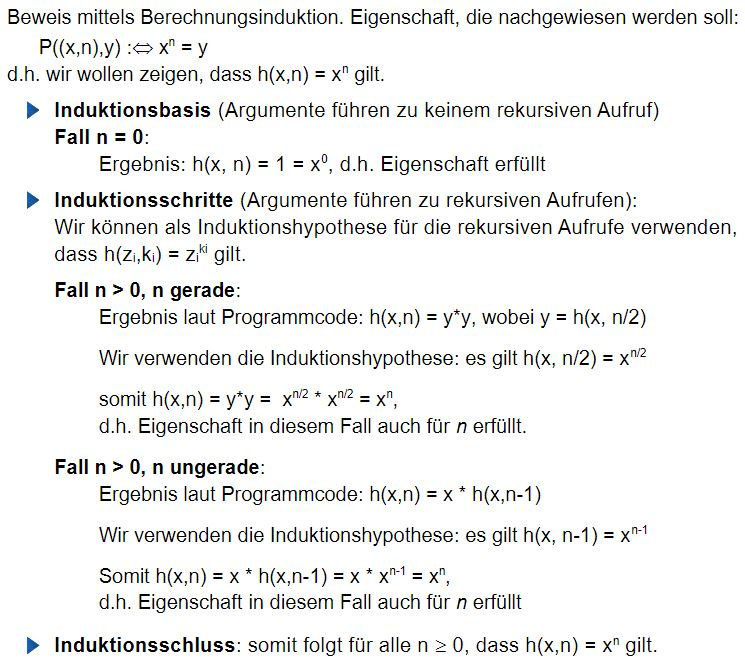
\includegraphics[width=0.8\textwidth]{graphics/3-2Korrektheit}
\section{Rekursive Berechnung der Potenzmenge}
\textbf{Beispiel:}
\\Menge: $M =\{a,b,c\}$
\\Potenzmenge: $\rho (M) = \{ \emptyset, \{a\}, \{b\}, \{c\}, \{a,b\}, \{a,c\}, \{b,c\}, \{a,b,c\} \}$
\subsection{Rekursiver Lösungsansatz}
a. in welchen einfach Fällen kann die Lösung direkt angegeben werden?
\\\tab der einfachste Fall ist die leere Menge $M = \emptyset$
\\\tab die leere Menge hat nur sich als Teilmenge $\rho(\emptyset) = \{\emptyset\}$
\\b. Wie können in nicht einfachen Fällen die Teilmengen bestimmt werden?
\\\tab Sei Menge $M = \{a_1,\ldots,a_{n-1},a_n\}$ nicht leer $(n\geq1)$
\begin{itemize}
  \item [1.] Wir wählen ein Element der Menge, z.B. $a_n$
  \item [2.] Es gibt nun zwei Arten von Teilmengen:
  \begin{itemize}
    \item [$T^+$] Teilmengen, die das Element $a_n$ enthalten
    \item [$T^-$] Teilmengen, die das Element $a_n$ nicht enthalten
  \end{itemize}
  Die Menge aller Teilmengen ist die Vereinigung von $T^+$ und $T^-$, d.h. $\rho(M) = T^+ \cup T^-$
  \\Die Menge $T^+$ kann nun rekursiv berechnet werden, indem wir $a_n$ aus $M$ entfernen und die Potenzmenge von $M$ berechnen.
  \\Die Menge $T^-$ ist die Potenzmenge von $M$ ohne $a_n$.
  \\Die Potenzmenge von $M$ ist also die Vereinigung von $T^+$ und $T^-$.
\end{itemize}
\textbf{Beispiel:} Wenn $M = \{a,b,c\}$
\\\tab Wähle z.B. c als Element:
\\\tab $T^-$: alle Teilmengen ohne c, also alle Teilmengen von $\{a,b\}$
\\\tab\tab $T^- =\{\emptyset,\{a\},\{b\},\{a,b\}\}$
\\\tab $T^+$: alle Teilmengen mit c, Nimm zu jeder Teilmenge von $T^-$ und füge c hinzu
\\\tab\tab $T^+ = \{\{c\},\{a,c\},\{b,c\},\{a,b,c\}\}$
\\\tab Insgesamt: $\rho(\{M\}) = T^+ \cup T^- =\{\emptyset,\{a\},\{b\},\{a,b\},\{c\},\{a,c\},\{b,c\},\{a,b,c\}\}$
\subsection{Algorithmischer Ansatz}
\textbf{Falls M leer} ($M = \emptyset$)
\\\tab leere Menge ist die einzige Teilmenge
\\\textbf{Falls M nicht leer} Wähle ein Element $a_n$ aus $M$
\\\tab Berechne Sammlung $T^-$ aller Teilmengen von M ohne $a_n$ (rekursiv)
\\\tab Berechne Sammlung $T^+$ aller Teilmengen, die $a_n$ enthalten:
\\\tab Nimm dazu jede Menge aus $T^-$ und bilde eine neue Menge, indem $a_n$ hinzugefügt wird
\\\tab Die Menge aller Teilmengen ist die Vereinigung von $T^+$ und $T^-$
\\\begin{lstlisting}
private static <E> Set<Set<E>> allSubsets(E[] arr,int maxIndex) {
Set<Set<E>> resultSet = new HashSet<Set<E>>();
if (maxIndex >= 0) {
  // Menge ist nicht leer, waehle letzes Element im gegebenen Bereich
E selected = arr[maxIndex];
  // Bilde rekursive alle Teilmengen ohne selected
Set<Set<E>> resultSet1 = allSubsets(arr, maxIndex - 1);
  // nimm jede dieser Mengen zum Ergebnis hinzu
resultSet.addAll(resultSet1);
  // bilde alle Teilmengen, die selected enthalten
for (Set<E> set1 : resultSet1) {
  // Erzeuge Kopie der Menge aus resultSet1 und nimm gewaehltes Element dazu
Set<E> set2 = new HashSet<E>(set1);
set2.add(selected);
  // fuege die ergaenzte Kopie zum Ergebnis hinzu
resultSet.add(set2);
}
} else {
  // Menge ist leer. Leere Menge hat nur leere Menge als einzige Teilmenge
Set<E> emptySet = new HashSet<>();
resultSet.add(emptySet);
}
return resultSet;
}
\end{lstlisting}
\section{Algorithmenprinzip ''Backtracking''}
\subsection{Grundidee ''Trial and Error''} 
\begin{itemize}
  \item [1.] Versuche eine Lösung zu finden
  \item [2.] Wenn die Lösung nicht passt, versuche eine andere Lösung
  \item [3.] Wenn keine Lösung passt, gehe zurück und versuche eine andere Lösung
\end{itemize}

\chapter{Analyse von Algorithmen}
\section{Korrektheit}
\subsection{Insertionsort}
\begin{itemize}
  \item Am Anfang des Arrays wird ein sortierter Bereich aufgebaut, in den nach und nach die folgenden Elemente 
  eingefügt werden (deshalb ''Insertionsort'').
  \item Am Anfang besteh der sortierte Bereich nur aus dem ersten Element $arr[0]$.
  \item In jedem Schritt wird ein Element $arr[i]$ aus dem unsortierten Bereich in den sortierten Bereich eingefügt.
  \item Wenn alle Elemente eingefügt wurden, ist das Array sortiert.
\end{itemize}
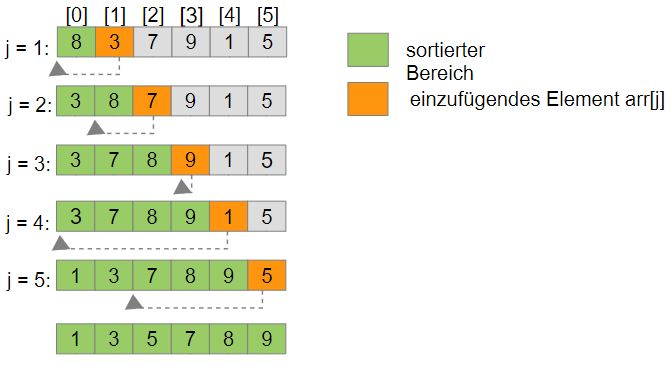
\includegraphics[width=0.65\textwidth]{graphics/insertionsort}
\\\textbf{Definition:}
\\ Enthält ein Array arr am Anfang die n Elemente $arr[0],arr[1],\dots,arr[n-1]$, so ist das Array sortiert, wenn gilt:
\begin{itemize}
  \item \textbf{Permutationen:} Die Elemente von arr sind eine Permutattion (Umordnung) der ursprünglichen 
  Elemente von $[0,n-1]$.
  \item \textbf{Monotonie:} Die Elemente von arr sind monoton steigend/fallend sortiert.
\end{itemize}
Mit \textbf{sortiert} ist sofern nicht anders angegeben immer \textbf{aufsteigend sortiert} gemeint.
\section{Komplexität von Algorithmen}
Komplexität bezeichnet den Ressourcenverbrauch von Algorithmen. Ressourcen sind dabei die Ausführungszeit und der Speicherbedarf.
\\Der Ressourcenbedarf hängt von mehreren Faktoren ab:
\begin{itemize}
  \item Umfang der Daten (Größe des Problems)
  \item Zusammensetzung der Daten (aktuelle Sortierung der Daten)
  \item Ausführungsgeschwindigkeit und Speicherbedarf bei der Ausführung
\end{itemize}
\subsection{Vorgehen bei der Laufzeitanalyse}
\begin{itemize}
  \item Bestimme für jede Anweisung $A_j$ des Programms die Häufigkeit $k_j$ der Ausführung.
  \item Die Gesamtkosten bei Problemgröße $n$ können dann so zusammengezählt werden:
  $T(n) = \sum_{A_j}^n k_j \cdot c_j$
  \\wobei $k_j$ die Häufigkeit für die Ausführung von Anweisung $A_j$ ist
  \\und $c_j$ die Einzel-Ausführungszeit für $A_j$ ist.
\end{itemize}
\subsection{Abhängigkeit von der Datenzusammensetzung}
\textbf{Best Case:} basiert auf Daten, die im Algorithmus eine minimale Anzahl von Schritten erfordern.
\\\textbf{Worst Case:} basiert auf Daten, die im Algorithmus eine maximale Anzahl von Schritten erfordern.
\\\textbf{Average Case:} basiert auf Daten, die im Algorithmus eine durchschnittliche Anzahl von Schritten erfordern.
\\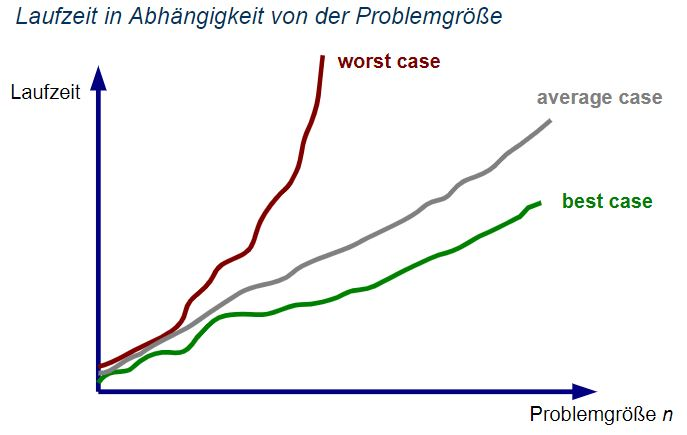
\includegraphics[width=0.65\textwidth]{graphics/Laufzeit}
\subsection{Häufig verwendete Größenordnungen}
\begin{itemize}
  \item $O (1)$: Konstante Laufzeit - elementare Operationen
  \item $O (\log n)$: Logarithmische Laufzeit - binäre Suche
  \item $O (n)$: Lineare Laufzeit - lineare Suche
  \item $O (n \log n)$: Logarithmische Laufzeit - schnelle Sortieralgorithmen
  \item $O (n^2)$: Quadratische Laufzeit - einfache Sortieralgorithmen
  \item $O (n^3)$: Kubische Laufzeit
  \item $O (c^n)$: Exponentielle Laufzeit
  \item $O (n!)$: Permutationen berechnen
\end{itemize}
\section{Komplexitätsanalyse wohlstrukturierter Algorithmen}
Unter wohlstrukturierten Algorithmen versteht man solche, die nur mit Hilfe von Sequenz (nacheinander ausführen),
Alternative (Fallunterscheidung) und Iteration (Schleife) definiert sind.
\subsection{Lineare Suche}
Bei der linearen Suche wird ein Array von links nach rechts durchsucht, bis das gesuchte Element gefunden wurde.
\\\begin{lstlisting}[language=Java]
public String sucheNummer(String suchname) {
  for (int i = 0; i < anzahl; i++) {
    if (liste[i].name.equals(suchname))
    return liste[i].nummer;} // gefunden
return null;} // nicht gefunden
\end{lstlisting}
\subsection{Binäre Suche}
Bei sortierten Daten kann der Bereich, in dem der gesuchte Schlüssel liegen kann, nach und nach immer wieder 
halbiert werden. Dieses Verfahren wird \textbf{binäre Suche} genannt.
\\\begin{lstlisting}[language=Java]
private String searchBinRek(String sname, int from, int to){
  if (to < from) {
    return null; //leerer Suchbereich, nichts gefunden
  } else {
  // Mitte des Suchbereichs berechnen
  int middle = (from + to) / 2;
  // Element in der Mitte vergleichen
  int res = suchname.compareTo(liste[middle].name);
    if (res < 0) {
    // in unterer Haelfte weitersuchen
    return searchBinRek(sname, from, middle-1);
    } else if (res > 0) {
    // in oberer Haelfte weitersuchen
    return searchBinRek(sname, middle+1, to);
    } else // (res == 0) {
    // Schluessel gefunden
  return liste[middle].number;
}}}
\end{lstlisting}

\chapter{Sortierverfahren}
\section{Vergleichsbasierte Sortierverfahren}
\textbf{Interne und Externe Sortierverfahren}
\begin{itemize}
  \item \textbf{Interne Sortierverfahren:} alle Datensätze passen in den Hauptspeicher.
  \item \textbf{Externe Sortierverfahren:} nur ein Teil der Datensätze passt in den Hauptspeicher.
\end{itemize}
Eine Ordnungsrelation heißt \textbf{total} wenn sie
\begin{itemize}
  \item die Eigenschaften einer Halbordnung erfüllt (reflexiv, transitiv, antisymmetrisch)
  \begin{itemize}
    \item reflexiv: $a \leq a$
    \item transitiv: $a \leq b$ und $b \leq c$ $\Rightarrow$ $a \leq c$
    \item antisymmetrisch: $a \leq b$ und $b \leq a$ $\Rightarrow$ $a = b$
  \end{itemize}
  \item und alle Werte miteinander vergleichbar sind.
\end{itemize}
\textbf{Vergleiche über Interface Comparable}
\begin{lstlisting}[language=Java]
public interface Comparable {
  int compareTo(Object o) throws ClassCastException;
}
\end{lstlisting}
wenn $x < y$ dann $x.compareTo(y) < 0$
\\wenn $x = y$ dann $x.compareTo(y) = 0$
\\wenn $x > y$ dann $x.compareTo(y) > 0$
\subsection{Laufzeitkomplexität von Selection-Sort}
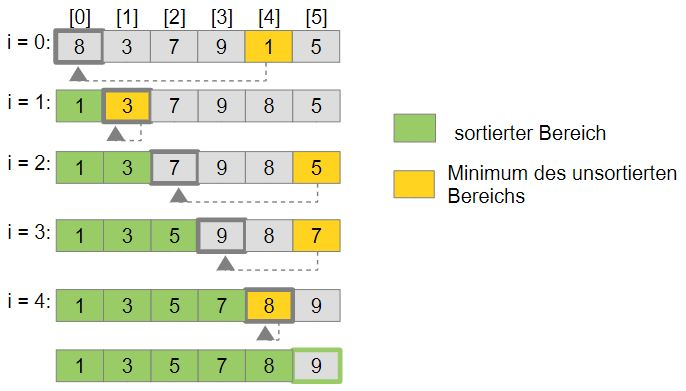
\includegraphics[width=0.65\textwidth]{graphics/Selectionsort}
\\\textbf{Worst Case = Best Case = Average Case:} $O(n^2)$
\subsection{Laufzeitkomplexität von Bubble-Sort}
\textbf{Best Case:} $O(n)$ - Daten sind schon aufsteigend sortiert
\\\textbf{Worst Case:} $O(n^2)$ - Daten sind absteigend sortiert
\\\textbf{Average Case:} $O(n^2)$
\section{Heapsort}
\subsection{Binäre Maximum-Heaps}
Ein \textbf{Maximum-Heap} ist ein binärer Baum, der folgende Eigenschaften erfüllt:
\begin{itemize}
  \item Der Baum ist fast vollständig - alle Ebenen bis auf die letzte sind vollständig.
  \item Für jeden Knoten gilt, dass der Schlüssel des Knotens größer oder gleich dem Schlüssel der Kinder ist.
\end{itemize}
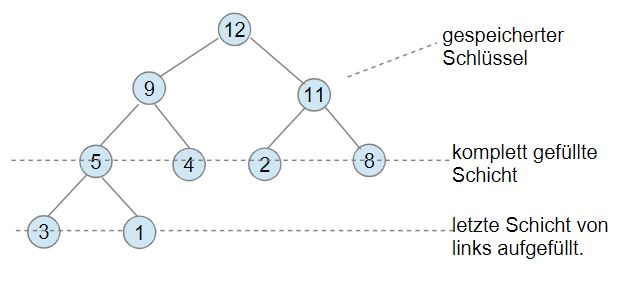
\includegraphics[width=0.65\textwidth]{graphics/maximum-heap}
\\\textbf{Speicherung eines fast vollständigen Baumes in einem Array:}
\\Die Wurzel wird an Index 0 abgelegt
\\Hat ein Knoten den Index $i$, so sind die Kinder an den Indizes $2i+1$ und $2i+2$ abgelegt.
\subsection{Soriteren mittels Heap}
Grundprinzip von Heapsort:
\\1. Heap aufbauen: Array wird in einen Maximum-Heap umgewandelt.
\\2. Heap abbauen, sortierten Bereich aufbauen:
\begin{itemize}
  \item Vertausche Wurzel a[0] und a[k], Maximum ist nun am Ende des Arrays.
  \item Heap-Eigenschaft wiederherstellen: Wurzel a[0] nach unten schieben, bis Heap-Eigenschaft 
  wiederhergestellt ist.
\end{itemize}
\subsection{Laufzeitkomplexität von Heapsort}
\textbf{''versenken'' (sink):} $O(\log n)$
\\\textbf{''erstelleMaxHeap'' (createMaxHeap):} $O(n \log n)$
\\\textbf{Heapsort:} $O(n \log n)$
\section{Rekursives Sortieren nach ''Teile und Herrsche''}
1. \textbf{Divide}: Besteht die Datenmenge aus mehr als einem Element, so wird sie in zwei Teilmengen zerlegt.
\\2. \textbf{Conquer}: Die Teilmengen werden rekursiv sortiert.
\\3. \textbf{Combine}: Die Teilmengen werden zusammengeführt.
\\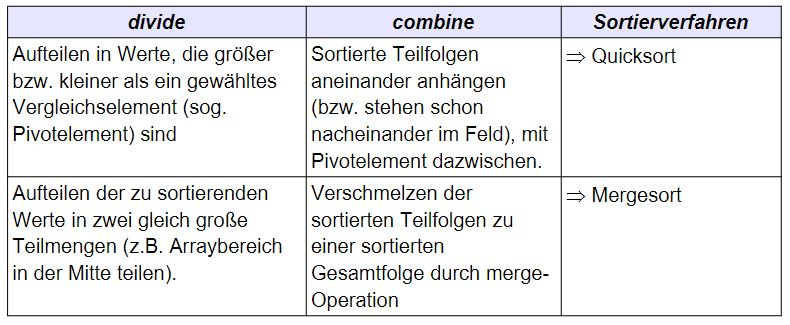
\includegraphics[width=0.65\textwidth]{graphics/sort-table}
\section{Quicksort}
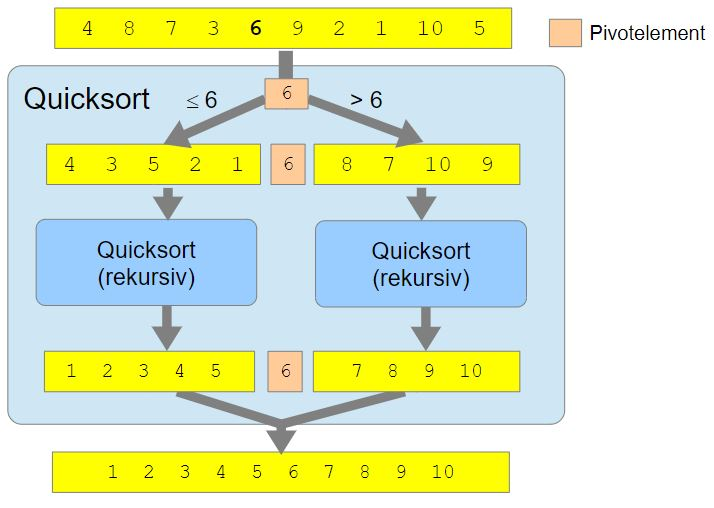
\includegraphics[width=0.65\textwidth]{graphics/Quicksort}
\subsection{Laufzeitkomplexität von Quicksort}
\textbf{Worst Case:} $O(n^2)$
\\\textbf{Best Case:} $O(n \log n)$
\\\textbf{Average Case:} $O(n \log n)$
\section{Mergesort}
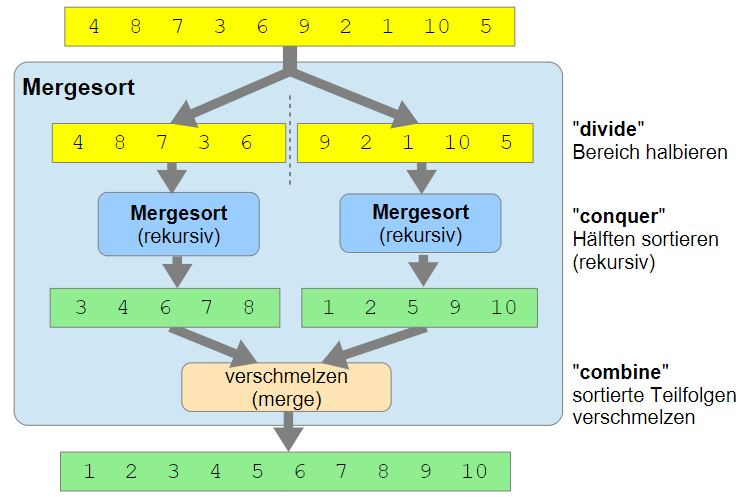
\includegraphics[width=0.65\textwidth]{graphics/Mergesort}
\\\begin{lstlisting}[language=Java]
void mergesort(double[] a, int von, int bis) {
  if (bis - von > 0) {
  //Mehr als ein Element zu sortieren
  //Daten in zwei Haelften aufteilen
  int mitte = (von + bis) / 2;
  //linke und rechte Haelfte sortieren
  mergesort(a, von, mitte);
  mergesort(a, mitte+1, bis);
  // Sortierte Teilfolgen a[von..mitte] und
  // a[mitte+1..bis] miteinender verschmelzen
  merge(a, von, mitte, bis);
  }
}
\end{lstlisting}
\subsection{merge - Verschmelzen sortierter Teilfolgen}
\begin{lstlisting}[language=Java]
void merge(double[] a, int links, int mitte, int rechts) {
  //Kopie der linken Haelfte a[links..mitte] erzeugen
  double[] tmpLinks = new double[mitte - links + 1];
  for (int i = 0; i < tmpLinks.length; i++) {
    tmpLinks[i] = a[links + i];
  }
  // Inhalt von tmpLinks (linker Teil) und a[mitte+1 .. rechts] zu
  // sortierter Gesamtfolge im Ergebnisbereich a[links..rechts] verschmelzen
  int indexLinks = 0;
  int indexRechts = mitte+1;
  int indexErgebnis = links;
  while (indexLinks < tmpLinks.length && indexRechts <= rechts) {
    // linke und rechte Teilfolge enthalten noch Elemente
    // nimm kleineren Wert von beiden Teilfolgen als naechsten Wert
    if (tmpLinks[indexLinks] <= a[indexRechts]) {
      a[indexErgebnis] = tmpLinks[indexLinks];
      indexLinks++;
    } else {
      a[indexErgebnis] = a[indexRechts];
      indexRechts++;
      }
    indexErgebnis++;
  }
  // falls nur noch linke Teilfolge Werte enthaelt (rechte Teilfolge aufgebraucht),
  // uebertrage sie in das Ergebnis
  while (indexLinks < tmpLinks.length) {
    a[indexErgebnis] = tmpLinks[indexLinks];
    indexErgebnis++;
    indexLinks++;
  }
  // falls linke Teilfolge abgearbeitet ist und nur noch rechte Teilfolge Werte
  // enthaelt, stehen diese schon richtig im Ergebnisfeld a und muessen nicht
  // mehr behandelt werden
}
\end{lstlisting}
\subsection{Laufzeitkomplexität von Mergesort}
\textbf{Worst Case = Best Case = Average Case:} $O(n \log n)$
\section{Eigenschaften der Sortierverfahren}
\textbf{Stabile Sortierverfahren:} Ein Sortierverfahren heißt stabil, wenn die relative Reihenfolge von Elementen,
deren Schlüssel gleich sind, während des Sortiervorgangs beibehalten wird wird.
\\Bubble-Sort, Insertion-Sort, Mergesort sind stabile Sortierverfahren.
\\Quicksort, Heapsort sind instabile Sortierverfahren.
\\Selectionsort ist ein instabiles Sortierverfahren, das aber stabil gemacht werden kann.
\\(für Arrays instabil -> für Listen stabil)
\subsection{Zusammenfassung der Sortierverfahren}
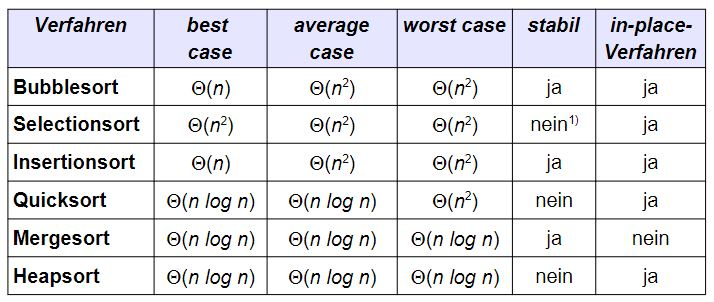
\includegraphics[width=0.65\textwidth]{graphics/sortierverfahren-table}
\section{Nicht-vergleichsbasierte Sortierverfahren}
Jedes vergleichsbasierte Sortierverfahren benötigt zum Sortieren von n
verschiedenen Schlüsseln im schlechtesten Fall (und auch im mittleren Fall)
$O(n \log n)$ Schlüsselvergleiche.
\subsection{Eigenschaften eines Entscheidungsbaums}
\begin{itemize}
  \item Ein Binärbaum repräsentiert die beim Suchen durchgeführten Vergleiche.
  \item Wurzelknoten repräsentiert den ersten Vergleich.
  \item Verzweigung nach links repräsentiert den Fall, dass der Vergleich wahr ist.
  \item Der Worst-Case ist der Pfad mit der größten Tiefe.
\end{itemize}
\subsection{Bucket-Sort}
\textbf{Idee:} Die Elemente werden in Buckets sortiert, die jeweils einen Bereich von Schlüsseln repräsentieren.
\\Die Buckets werden dann einzeln sortiert und anschließend zusammengeführt.
\\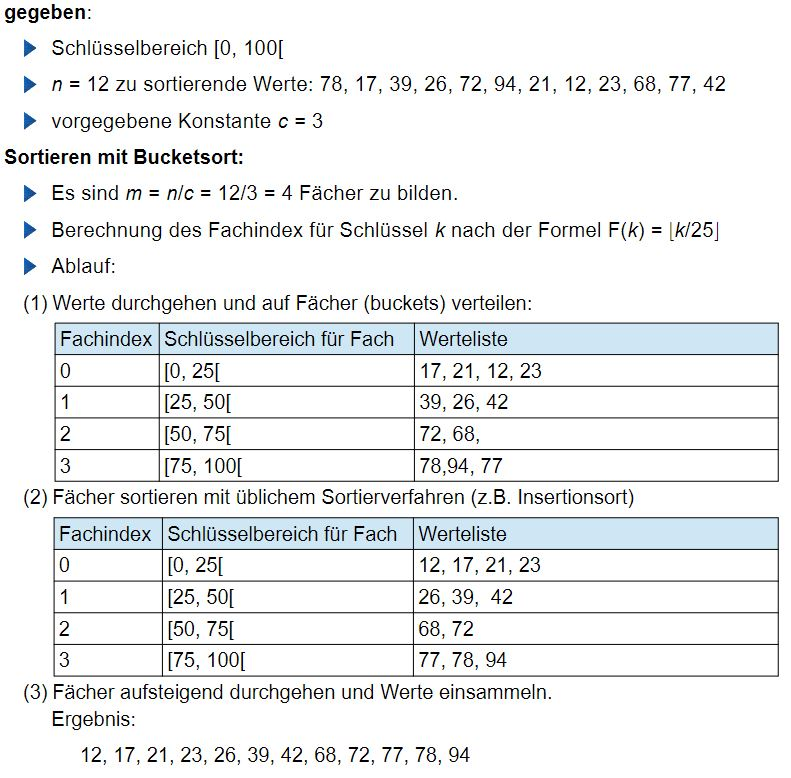
\includegraphics[width=0.65\textwidth]{graphics/Bucketsort}
\\\textbf{Laufzeitkomplexität:} 
\\\textbf{Best Case = Average Case:} $O(n)$
\\\textbf{Worst Case} $O(n^2)$
\subsection{Radix-Sort}
Wiederhole für jede Stelle p der insgesamt d Stellen, von der niederwertigsten
Stelle rechts bis zur höchstwertigen Stelle links jeweils folgende Partitioniserungs-
und Sammelphase
\\(1) Partitionierungsphase: Gehe die Wertefolge durch und ordne sie
entsprechend dem Zeichen an der Stelle p in das zugehörige Fach ein.
\\wichtig: neue Elemente werden hinten an die Fachliste angehängt!
\\(2) Sammelphase: Die Einträge aus den Fächern aufsammeln und wieder in
eine lineare Folge bringen
\\- bei Fach mit niedrigstem Wert beginnen
\\- die im Fach vorgegebene Reihenfolge muss beibehalten werden
\\Diese Folge wird dann beim nächsten Durchgang für die Partitionierung
verwendet.
\\Nach d Durchgängen durch alle Stellen sind die Daten richtig sortiert.
\\\textbf{Laufzeitkomplexität:}
\\Best Case = Worst Case = Average Case: $O(d \cdot n) = O(n)$

\chapter{Einfache Datenstrukturen}
\section{Abstrakte und konkrete Datenstrukturen}
\textbf{Abstrakte Datentypen (ADT):}
\\Ein ADT definiert eine Datenstruktur unabhängig von ihrer konkreten Implementierung.
\\\textbf{Konkrete Datenstrukturen:}
\\Ein konkreter Datentyp ist die Implementierung eines ADT.
\section{Abstrakter Datentyp Stack}
\textbf{Stack:} Eine Sammlung von Elementen, die nach dem LIFO-Prinzip (Last In First Out) verwaltet wird.
\\\begin{lstlisting}[language=Java]
public interface Stack {
  void push(Object elem); // Element oben auf dem Stack ablegen
  Object pop() throws EmptyStackError;
  // oberstes Element des Stacks entnehmen und zurueckgeben
  boolean isEmpty(); // prueft, ob Stack leer ist
}
\end{lstlisting}
\section{Konkreter Datentyp ArrayStack}
Bei Stacks kann man noch zwei Varianten unterscheiden:
\\ob sie eine begrenzte Kapazität haben oder sie unbeschränkt wachsen können.
\\\textbf{Laufzeitkomplexität für ArrayStack mit begrenzter Kapazität:} $O(1)$
\section{Amortisierte Laufzeitanalyse}
Die Laufzeit eines Algorithmus wird über mehrere Operationen hinweg betrachtet.
\section{Abstrakter Datentyp Warteschlange}
Eine Queue ist eine Sammlung von Elementen, die nach dem FIFO-Prinzip (First In First Out) verwaltet wird.
\\\begin{lstlisting}[language=Java]
public interface Queue {
  void enqueue(Object elem); // fuege Element vorne ein
  Object dequeue() throws EmptyQueueError;
  // entnimmt Element hinten
  boolean isEmpty(); // pruefen, ob Wartschlange leer ist
}
\end{lstlisting}
\section{Konkreter Datentyp Ringpuffer}
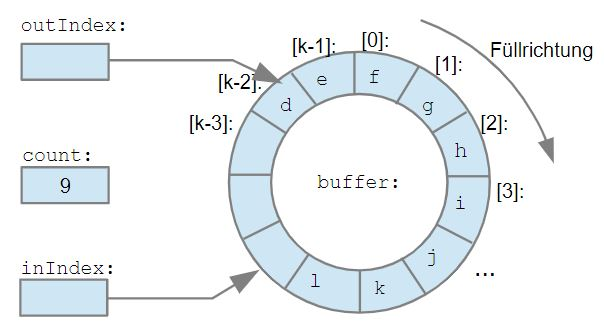
\includegraphics[width=0.65\textwidth]{graphics/Ringpuffer}
\\\textbf{Laufzeitkomplexität:} $O(1)$S
\section{Abstrakter Datentyp Prioritätswarteschlange}
Eine Prioritätswarteschlange ist eine Datenstruktur zur Verwaltung eine Sammlung von Einträgen,
wobei die Einträge jeweils mit einer Priorität versehen sind, die bestimmt, in welcher
Reihenfolge die Elemente entnommen werden.
\\\textbf{Grundoperationen:}
\\ insert(x) - Einfügen eines ELements (Schlüssel in x enthalten)
\\ extractMin() - Rückgabe \& Entfernen des Elements mit kleinstem Schlüssel --> höchste Priorität
\section{Konkreter Datentyp verkettete Liste}
Die Datenstruktur, die eine Folge von Einträgen speichert, wird durch einzelne Knotenobjekte realisiert, die
jeweils über eine Referenz auf einen Nachfolger verweisen. Durch Anhängen,
Entfernen oder Umhängen einzelner Knotenobjekte kann die Wertefolge dynamisch in
Umfang und Reihenfolge verändert werden.
\\ Einfach verkette Liste mit first- und last-Referenz
\\ Doppelt verkettete Liste mit first- und last-Referenz
\section{Abstrakter Datentyp Double-Ended-Queue (Deque)}
Eine Deque ist eine Warteschlange, bei der an beiden Enden Elemente eingefügt und entfernt werden können.
\section{Zusammenfassung: Anwendung verketter Listen}
\begin{itemize}
  \item Stacks
  \\ push(v), pop() - $O(1)$
  \item Queues
  \\ enqueue(v), dequeue() - $O(1)$
  \item Double-Ended-Queues
  \\ insertFirst(v), insertLast(v), removeFirst(), removeLast() - $O(1)$
\end{itemize}

\chapter{Suchbäume}
\section{Abstrakte Datentypen Map und Set}
\subsection{Abstrakter Datentyp Map}
Ein Map ist eine Sammlung von Schlüssel-Wert-Paaren, die nach den Schlüsseln verwaltet wird.
\\ Grundoperationen:
\\ put(k,v) - Einfügen eines Schlüssel-Wert-Paares - v wird unter dem Schlüssel k abgelegt
\\ get(k) - Rückgabe des Wertes, der unter dem Schlüssel k abgelegt ist
\\ delete(k) - Entfernen des Schlüssel-Wert-Paares mit Schlüssel k
\subsection{Abstrakter Datentyp Set}
Ein Set ist eine Sammlung von Elementen, die nach den Elementen verwaltet wird.
\\ - Ein Element kann höchstens einmal im Set vorkommen
\\ Grundoperationen:
\\ add(x) - Einfügen eines Elements
\\ remove(x) - Entfernen eines Elements
\\ contains(x) - Prüfen, ob ein Element im Set enthalten ist
\\ isEmpty() - Prüfen, ob das Set leer ist
\\ size - Anzahl der Elemente im Set
\section{Binäre Bäume}
\subsection{Implementierung eines binären Baumes}
\begin{lstlisting}[language=Java]
public class TreeNode {
  Object value; // Wert des Knotens
  TreeNode left, right; // linke und rechte Teilbaeume
  public TreeNode(Object value, TreeNode left, TreeNode right) {
    this.value = value;
    this.left = left;
    this.right = right;
  }
  public TreeNode(Object value) { // erzeugt Blattknoten
    this(value, null, null);
  }
}
\end{lstlisting}
\textbf{Traversierung eines binären Baumes:}
\\ Inorder: links, Wurzel, rechts - sortiert
\\ Preorder: Wurzel, links, rechts - für Ausdrücke
\\ Postorder: links, rechts, Wurzel - für Ausdrücke
\section{Binäre Suchbäume}
Ein Suchbaum ist ein binärer Baum, bei dem für jeden Knoten p des Baums gilt:
\\ - Alle Schlüssel im linken Teilbaum von p sind kleiner als der Schlüssel von p
\\ - Alle Schlüssel im rechten Teilbaum von p sind größer als der Schlüssel von p
\\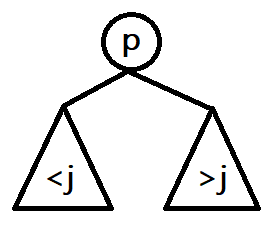
\includegraphics[width=0.65\textwidth]{graphics/Suchbaum}
\subsection{Suchbaum-Operationen}
\textbf{Rekursive Suche:}
\begin{lstlisting}
Suche nach Knoten mit Key k
- falls Baum leer: Suche fehlgeschlagen
- falls Baum nicht leer, Wurzel hat Key w:
  - falls w = k: Suche erfolgreich
  - falls k < w: Suche im linken Teilbaum
  - falls k > w: Suche im rechten Teilbaum
\end{lstlisting}
\textbf{Einfügen eines Knotens:}
\begin{lstlisting}
Einfuegen eines Knotens mit Key k
- falls Baum leer: neuer Knoten wird Wurzel
- falls Baum nicht leer, Wurzel hat Key w:
  - falls k < w: Einfuegen im linken Teilbaum
  - falls k > w: Einfuegen im rechten Teilbaum
\end{lstlisting}
\textbf{Entfernen eines Knotens:}
\begin{lstlisting}
Entfernen eines Knotens mit Key k
- falls Baum leer: Entfernen fehlgeschlagen
- falls Baum nicht leer, Wurzel hat Key w:
  - falls w = k: Entfernen erfolgreich
  - falls k < w: Entfernen im linken Teilbaum
  - falls k > w: Entfernen im rechten Teilbaum
\end{lstlisting}
\subsection{Laufzeitkomplexität von binären Suchbäumen}
\begin{itemize}
  \item Suche: $O(\log n)$ - Worst Case: $O(n)$
  \item Einfügen: $O(\log n)$ - Worst Case: $O(n)$
  \item Entfernen: $O(\log n)$ - Worst Case: $O(n)$
\end{itemize}
\section{Grundprizip balancierter Suchbäume}
Bäume werden durch Rotationen so verändert, dass die Tiefe der Teilbäume möglichst gleich bleibt.
\section{AVL-Bäume}
\subsection{Balancefaktor und AVL-Ausgleich}
\textbf{Balancefaktor:}
\\\tab $B_x = height(left(x)) - height(right(x))$
\\ Ein Blatt hat Balancefaktor 0, da die Höhe des linken und rechten Teilbaums gleich ist.
\\\textbf{AVL-Ausgleich:}
\\ Ein AVL-Baum ist ein binärer Suchbaum, bei dem für jeden Knoten p gilt:
\\ - Der Balancefaktor von p ist -1, 0 oder 1
\\\textbf{Höhe eines AVL-Baums:}
\\\tab $h = O(\log n)$
\subsection{Suche in AVL-Bäumen}
Die Laufzeitkomplexität von AVL-Bäumen ist im Worst und Average Case $O(\log n)$.
\subsection{Rotationen in Suchbäumen}
Eine Links- oder Rechtsrotation ist eine Rotation, bei der ein Knoten p um eine Ebene nach links oder rechts verschoben wird.
\\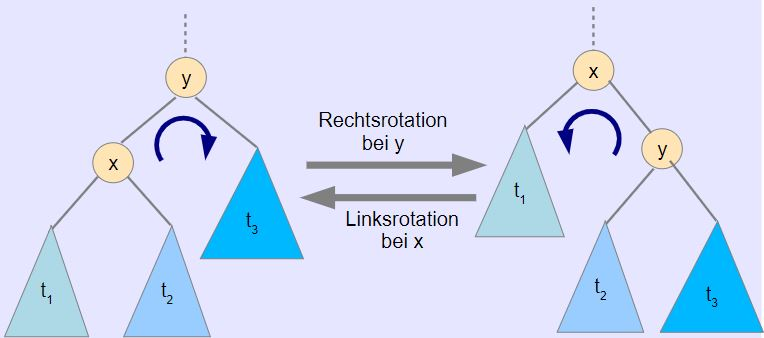
\includegraphics[width=0.65\textwidth]{graphics/Rotationen}
\subsection{Einfügen in AVL-Bäumen}
\begin{lstlisting}
(1) Suche wie beim Suchbaum die Position k (als Blatt)
(2) Einfuegen des neuen Knotens k
(3) Falls Balancefaktor von k ungleich 0:
  - Falls Balancefaktor von k ungleich Balancefaktor von p:
    - Falls Balancefaktor von k = -1 und Balancefaktor von p = -1:
      - Rechtsrotation um p
    - Falls Balancefaktor von k = 1 und Balancefaktor von p = 1:
      - Linksrotation um p
  - Falls Balancefaktor von k gleich Balancefaktor von p:
    - Falls Balancefaktor von k = -1 und Balancefaktor von p = -1:
      - Rechtsrotation um p
      - Linksrotation um q
    - Falls Balancefaktor von k = 1 und Balancefaktor von p = 1:
      - Linksrotation um p
      - Rechtsrotation um q
\end{lstlisting}
\subsection{Entfernen in AVL-Bäumen}
\begin{lstlisting}
(1) Suche den zu entfernenden Knoten k und merke den Pfad von der Wurzel zu k.
(2) Falls Knoten k Blatt ist oder nur ein Kind hat:
        Entferne k wie in einem Suchbaum
    Falls Knoten k zwei Kinder hat:
        Suche im linken Baum von k den groessten Knoten l und ersetze k durch l
(3) Verfolge den Pfad zur Wurzel und aktualisiere die Balancefaktoren und rotiere bei Bedarf
(4) Wenn AVL-Ausgleich verletzt ist --> Einfach- bzw Doppelrotation
\end{lstlisting}
\subsection{Laufzeitkomplexität für AVL-Bäume}
Worst \& Average Case:
\begin{itemize}
  \item Suche: $O(\log n)$
  \item Einfügen: $O(\log n)$
  \item Entfernen: $O(\log n)$
\end{itemize}
\section{B-Bäume}
Es handelt sich dabei um Mehrwegbäume, bei denen ein einzelner Knoten eine (sortierte) Folge von Schlüsseln
speichert und es auch entsprechendmehr als zwei Kinder geben kann.
\subsection{Definition}
Für einen B-Baum der Ordnung m ($m \geq 2$) gilt:
\\\textbf{Struktur des Baums:}
\begin{itemize}
  \item [(1)] Alle Blätter haben die gleiche Tiefe - Abstand zur Wurzel
  \item [(2)] Enthält ein innerer Knoten j Schlüssel, dann hat er j+1 Kinder
  \item [(3)] Jeder Knoten enthält maximal $2m-1$ Schlüssel
  \item [(4)] Jeder Knoten enthält mindestens $m-1$ Schlüssel
  \item [(5)] Die Wurzel enthält mindestens einen Schlüssel
\end{itemize}
\textbf{Geordnete Speicherung:}
\\ Enthält ein Knoten die Schlüssel $k_1, k_2, \dots, k_n$, dann gilt:
\begin{itemize}
  \item [(6)] Die Schlüssel sind aufsteigend geordnet
  \item [(7)] Für alle Werte x im ersten Unterbaum des Knotens gilt: $x < k_1$
  \item [(8)] Sind $k_{j-1}$ und $k_j$ zwei aufeinanderfolgende Schlüssel, dann gilt: $k_{j-1} < x < k_j$
  \item [(9)] Für alle Werte x im letzten Unterbaum des Knotens gilt: $x > k_j$
\end{itemize}
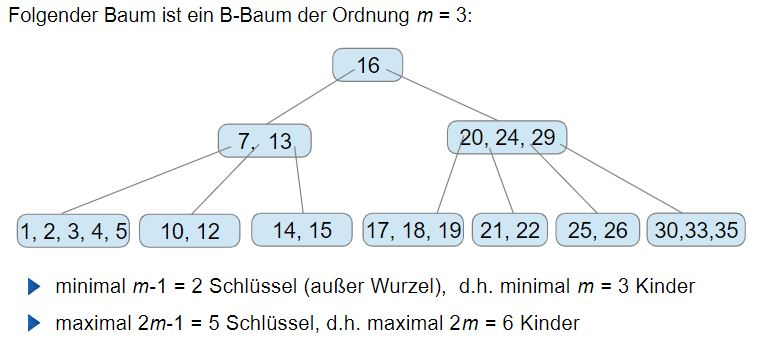
\includegraphics[width=0.65\textwidth]{graphics/B-Baum}
\subsection{Höhe von B-Bäumen}
$h \leq [log_m(\frac{n+1}{2})]$
\subsection{2-3-4 Bäume}
B-Bäume der Ordnung $m=2$ werden auch 2-3-4 Bäume genannt.
\begin{itemize}
  \item Jeder Knoten kann zwei, drei oder vier Nachfolger haben
  \item Jeder Knoten kann einen, zwei oder drei Schlüssel enthalten
\end{itemize}
\subsection{Suche in B-Bäumen}
\begin{lstlisting}
- Man beginnt mit dem Wurzelknoten
- In einem Knoten kann mit bin. Suche nach dem Wert gesucht werden
- Wenn der Wert gefunden wurde, ist die Suche beendet
- Wenn der Wert nicht gefunden wurde, wird der entsprechende Unterbaum
  durchsucht
- Wenn der Wert nicht gefunden wurde, ist die Suche beendet
\end{lstlisting}
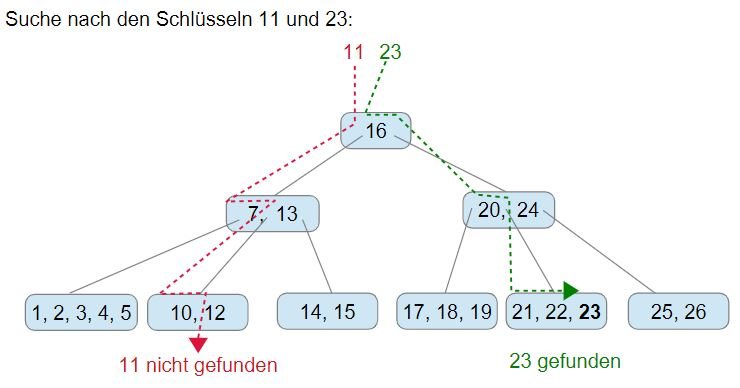
\includegraphics[width=0.65\textwidth]{graphics/B-Baum-Suche}
\subsection{Einfügen in B-Bäumen}
\begin{lstlisting}
- Ausgehend von der Wurzel das passende Blatt fuer Key k suchen
- Neuen Key k an der richtigen Stelle in den Blattknoten einfuegen
  - Falls Blatt schon voll ist, muss der Knoten aufgeteilt werden
\end{lstlisting}
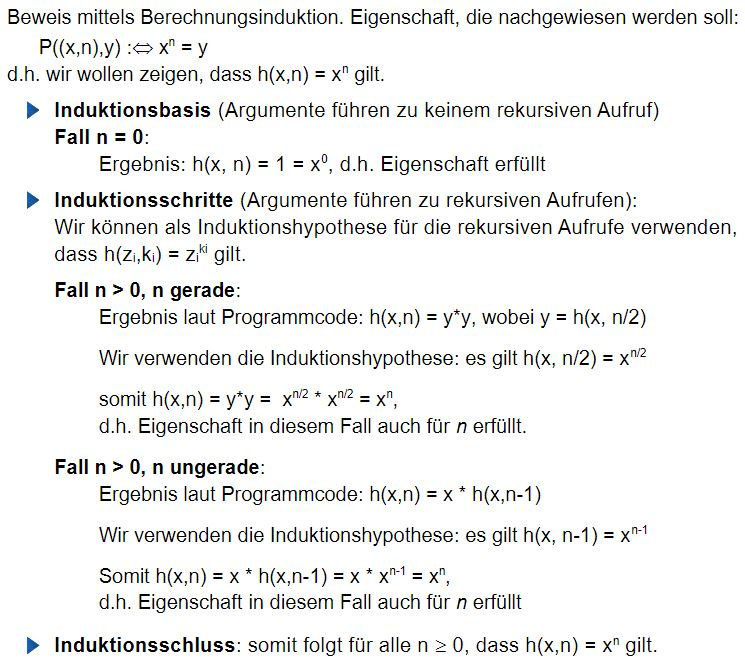
\includegraphics[width=0.65\textwidth]{graphics/Splitten}
\subsection{Entfernen in B-Bäumen}
Schlüssel liegt im Blatt:
\\ Der Schlüssel wird entfernt und der Knoten wird ggf. zusammengeführt.
\\Schlüssel liegt nicht im Blatt:
\\ Der Schlüssel wird durch seinen direkten Vorgänger (Maximum davor) oder direkten Nachfolger (Minimum danach) ersetzt und der Knoten wird ggf. zusammengeführt.
\subsection{Laufzeitkomplexität für B-Bäume}
Worst \& Average Case:
\begin{itemize}
  \item Suche: $O(\log n)$
  \item Einfügen: $O(\log n)$
  \item Entfernen: $O(\log n)$
\end{itemize}
\section{Rot-Schwarz Bäume}
Binäre Suchbäume haben den Vorteil, dass sie einfach zu implementieren sind und ein einfaches Suchen und Traversieren ermöglichen.
\\B-Bäume haben den Vorteil, dass sie immer weitgehend ausbalanciert sind.
\\Rot-Schwarz Bäume kombinieren die Vorteile der beiden.
\subsection{Definition}
\begin{itemize}
  \item Jeder Knoten ist rot oder schwarz
  \item Die Wurzel ist schwarz
  \item Jeder rote Knoten hat nur schwarze Kinder
  \item Jeder Nil-Knoten unter einem Blatt ist per Definition schwarz
  \item Für jeden Knoten k gilt: Jeder Pfad von k zu einem Blatt hat die gleiche Anzahl an schwarzen Knoten
  \item Nil-Knoten: Knoten ohne Schlüssel - nur als Platzhalter (schwarz)
\end{itemize}
\textbf{Höhe von Rot-Schwarz Bäumen:} $h \leq 2 \cdot [log_2(n+1)]$
\subsection{Suche in Rot-Schwarz Bäumen}
Die Suche erfolgt wie bei binören Suchbäumen - die Farbe der Knoten spielt dabei keine Rolle.
\\Worst Case: $O(\log n)$
\subsection{Einfügen in Rot-Schwarz Bäumen}
Beim Einfügen neuer Schlüssel kann zunächst, wie bei binären Suchbäumen üblich, vorgegangen werden und der
Wert als neues Blatt an passender Stelle eingehängt werden.
\\Danach muss die Farbe des Knotens und die Farbe der Kinder geprüft werden.
\begin{itemize}
  \item Wird ein neues Blatt als roter Knoten eingefügt führt das ggf. zu einem Rot-rot-Problem
  \item Wird ein neues Blatt als schwarzer Knoten eingefügt, zerstört das die Eigenschaft, 
  dass auf allen Pfaden von der Wurzel zu einem Blatt die gleiche Anzahl an schwarzen Knoten liegt
  \item Probleme mit roten Blättern sind leichter zu lösen als mit schwarzen Blättern
\end{itemize}
\textbf{Prinzipielle Vorgehensweise:}
\begin{lstlisting}
- neuen Key als Blatt einfuegen - Farbe rot (2 schwarze Nil-Knoten)
- Falls Elternknoten rot --> Korrekturen 
- Falls am Ende Wurzel rot --> Farbe schwarz
\end{lstlisting}
\textbf{Reorganisation durch Insertion Fixup:}
\\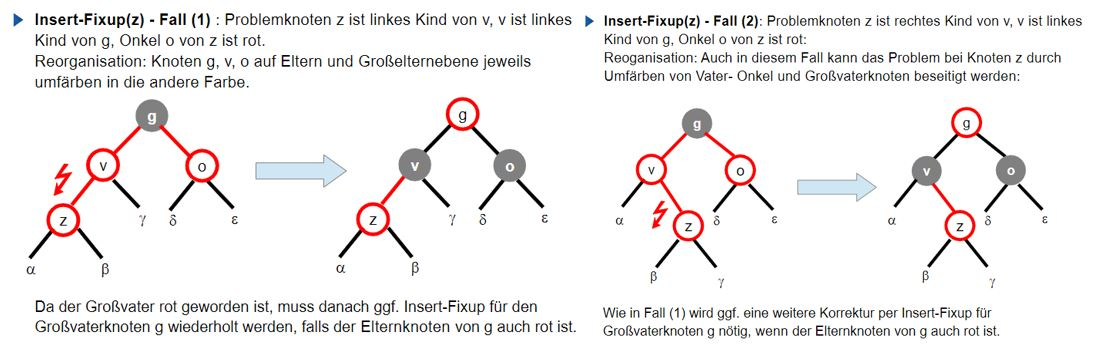
\includegraphics[width=1\textwidth]{graphics/Fixup1}
\\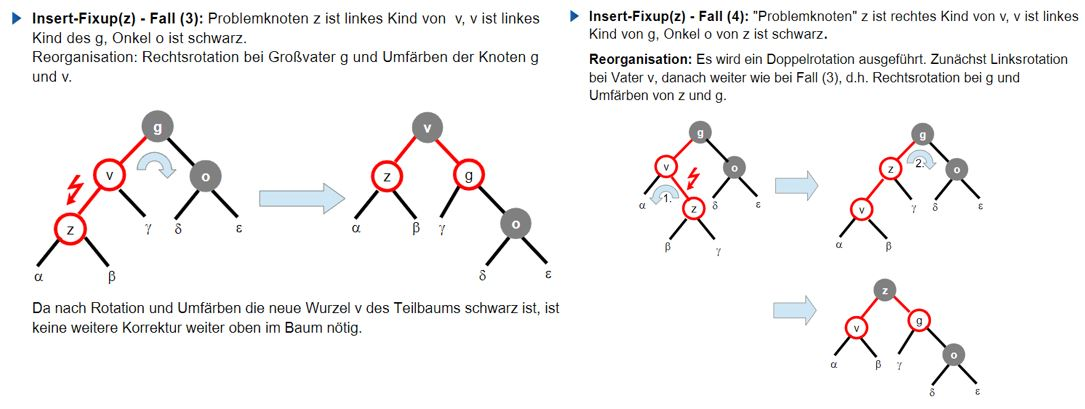
\includegraphics[width=1\textwidth]{graphics/Fixup2}
\subsection{Laufzeitkomplexität für Rot-Schwarz Bäume}
Worst \& Average Case:
\\- Einfügen: $O(\log n)$
\\- Entfernen: $O(\log n)$
\\- Suche: $O(\log n)$
\section{Tries}
Jeder Knoten enthält ein Array von der Größe des Alphabets M mit Referenzen auf die zugehörigen Teilbäume.
\\Jeder Knoten kann außer den Referenzen auf die Kinderknoten auch eine Zeichenkette speichern.
\\\textbf{Binäre Tries:}
Binäre Tries sind eine Spezialfall für das binäre Alphabet M = {0,1}. Die Schlüsselwerte sind somit Bitfolgen.
Da es pro Zeichen einen Nachfolger geben kann, ergibt sich ein Binärbaum.
\subsection{Suche in Tries}
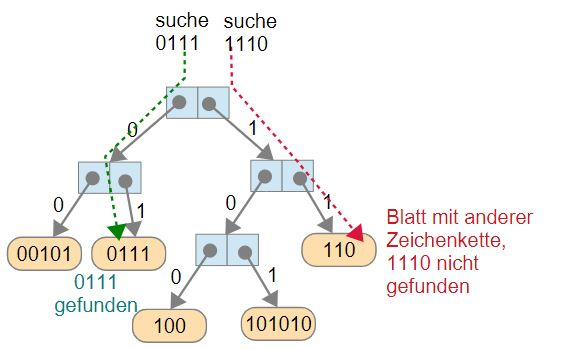
\includegraphics[width=0.7\textwidth]{graphics/trie-suche}
\subsection{Einfügen in Tries}
\begin{lstlisting}
- nach Zeichenkette suchen - falls vorhanden, fertig
- falls nicht vorhanden, neue Zeichenkette einfuegen
  - Endet Suche mit leerer Referenz eines inneren Knotens, wird dort neue Zeichenkette eingefuegt
  - Endet Suche an einem Blatt, das ein anderes Wort speichert --> Blatt wird aufgeteilt
  - Endet Suche bei innerem Knoten wird dort neue Zeichenkette eingefuegt
\end{lstlisting}

\chapter{Hashtabellen}
\section{Grundprinzip Hashing}
Die Einträge werden in einem Array fester Größe gespeichert.
\\ Bei Maps besteht jeder Eintrag aus Schlüssel und Wert. Bei Sets besteht der Eintrag nur aus dem Schlüssel.
\section{Hashfunktionen}
Die Funktion muss schnell berechenbar sein, möglichst wenig Adresskollisionen verursachen und alle Adressen gleich wahrscheinlich besuchen.
\subsection{Division-Rest-Methode}
\textbf{Hashfunktion nach Division-Rest-Methode:} $h(k) = k mod m$
\\Schlecht geeignet ist eine 2er-Potenz $2^j$ als Größe des Arrays, da dann nur die $j$-niedrigsten Bits des Schlüssels betrachtet werden.
\\Eine bessere Wahl ist eine Primzahl $p$ als Größe des Arrays, da dann alle Schlüsselwerte betrachtet werden.
\subsection{Multiplikationsmethode}
\textbf{Hashfunktion nach Multiplikationsmethode:} $h(k) = \lfloor m \cdot (F \cdot k - \lfloor F \cdot k \rfloor ) \rfloor$
\\Dabei ist $F$ eine irrationale Zahl.
\section{Adresskollisionen}
Eine Adresskollision tritt auf, wenn zwei Schlüsselwerte auf die gleiche Adresse abgebildet werden. --> Hashfunktion muss so gewählt werden, dass dies möglichst selten vorkommt.
\subsection{Wahrsccheinlichkeit für Adresskollisionen}
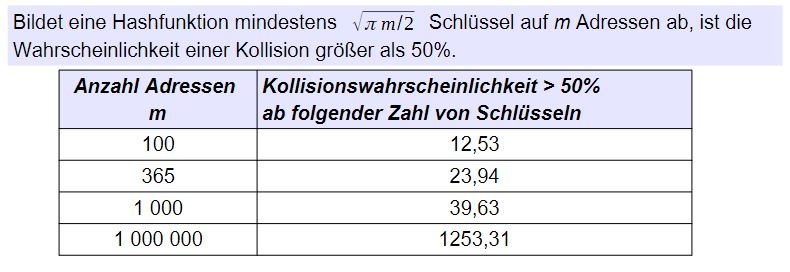
\includegraphics[width=0.7\textwidth]{graphics/kollisionen}
\subsection{Auflösung von Adresskollisionen}
\textbf{Verkettung der Überläufer:}
\\Es wird ein Überlaufbereichs außerhalb der Hashtabelle verwenden (typischerweise als verkettete Listen 
implementiert), so dass zu einer Adresse mehrere Einträge gespeichert werden können.
\\\textbf{Hashing mit offener Adressierung:}
\\Ist beim Eintragen eine Adresse bereits belegt, wird nach einer sog. Sondierungsregel eine Ersatzposition 
innerhalb der Hashtabelle gesucht. Beim Suchen muss dann in gleicher Weise auch
berücksichtigt werden, an welchen Ersatzpositionen entsprechend der Sondierungsregel der Eintrag gespeichert sein könnte.
\\\textbf{Belegungsfaktor $\beta$:}
\\\tab $\beta = \frac{n}{m}$ --> Anzahl der Einträge $n$ durch Größe der Hashtabelle $m$.
\section{Hashing mit Verkettung der Überläufer}
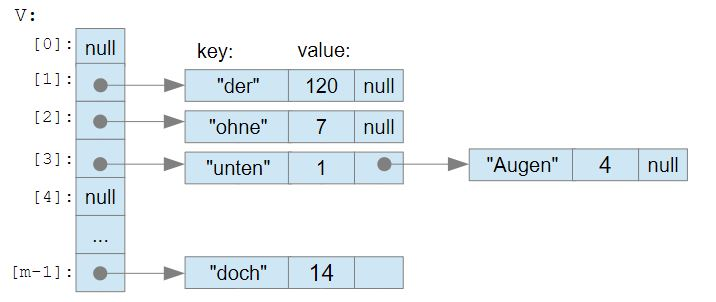
\includegraphics[width=0.7\textwidth]{graphics/verkettung}
\subsection{Laufzeitanalyse}
\textbf{Einfügen, Suchen, Löschen:}
\\- Worst Case: $O(n)$
\\- Average Case: $O(1)$
\section{Hashing mit offener Adressierung}
Lektion 19 ab 8.5 //TODO

\chapter{Das Java-Collection-Framework}
\section{Hashtabellen in Java}
\subsection{Klassen in Package java.util}
\begin{tabular}{|l|l|}
\hline
\textbf{Klasse} & \textbf{Beschreibung} \\
\hline
\texttt{HashMap} & \texttt{Map}-Implementierung mit Hashing \\
\texttt{HashSet} & \texttt{Set}-Implementierung mit Hashing \\
\texttt{Hashtable} & \texttt{Map}-Implementierung mit Hashing \\
\hline
\end{tabular}
\section{Collections}
Eine Collection ist eine Sammlung von Objekten mit folgenden Operationen:
\begin{itemize}
  \item \texttt{add(E e)}: Fügt ein Element hinzu
  \item \texttt{contains(Object o)}: Prüft, ob ein Element enthalten ist
  \item \texttt{remove(Object o)}: Entfernt ein Element
\end{itemize}
\begin{lstlisting}
public interface Collection<E> {
  boolean add(E o);
  boolean contains(Object o);
  boolean remove(E o);
  boolean isEmpty();
  int size();
  Iterator<E> iterator();
  ...
}
\end{lstlisting}
\subsection{Abstrakte Datentypen}
\begin{itemize}
  \item List - Liste
  \item Queue - Warteschlange
  \item Set - Menge
\end{itemize}
\subsection{Konkrete Implementierungen}
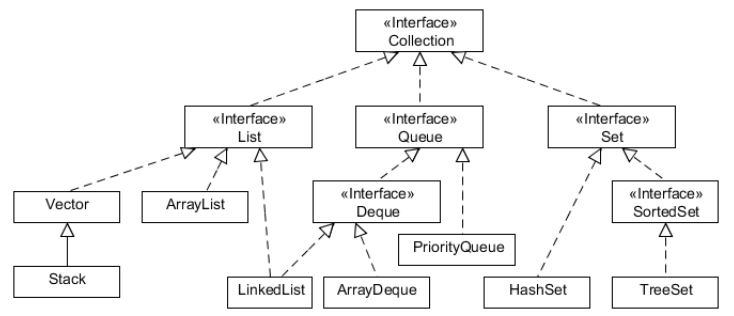
\includegraphics[width=0.7\textwidth]{graphics/Collections}
\\\textbf{Listen:}
\begin{itemize}
  \item LinkedList - Doppelt verkettete Liste (nicht thread-safe)
  \item ArrayList - Array mit dynamischer Größe (nicht thread-safe)
  \item Vector - Array mit dynamischer Größe (thread-safe)
  \item Stack - Unterklasse von Vector
\end{itemize}
\textbf{Queues:}
\begin{itemize}
  \item PriorityQueue - Warteschlange mit Priorität
  \item ArrayDeque - Ringpuffer mit dynamischer Größe (nicht thread-safe)
  \item LinkedList - Doppelt verkettete Liste (nicht thread-safe)
\end{itemize}
\textbf{Sets:}
\begin{itemize}
  \item HashSet - dynamische Hashtabelle
  \item TreeSet - Rot-Schwarz-Baum 
\end{itemize}
\section{Maps}
Eine Map ist eine Sammlung von Schlüssel-Wert-Paaren.
\subsection{Implementierungen}
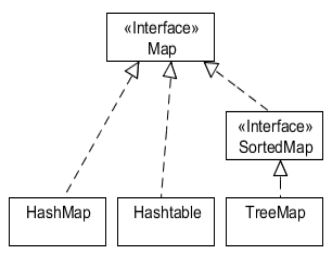
\includegraphics[width=0.7\textwidth]{graphics/Maps}
\begin{itemize}
  \item HashMap - dynamische Hashtabelle (nicht thread-safe)
  \item Hashtable - HashMap (thread-safe)
  \item TreeMap - Rot-Schwarz-Baum, Schlüssel müssen Comparable sein
\end{itemize}
\section{Iteratoren}
\textbf{Definition:} Ein Objekt, das zu einer Datensammlung gehört und das erlaubt, 
\\- alle Elemente der Sammlung nacheinander zu durchlaufen.
\\- ohne Kenntnis der konkreten Implementierung der Sammlung.
\begin{lstlisting}[language=Java]
public interface Iterator<E> {
  boolean hasNext(); // gibt true zurueck, wenn noch ein Element vorhanden ist
  E next(); // liefert das naechste Element
  void remove(); // entfernt das aktuelle Element
}
\end{lstlisting}
\section{For-each-Schleife für Collections}
\begin{lstlisting}[language=Java]
for (E e : collection) {
  // e ist das aktuelle Element
}
\end{lstlisting}

\chapter{Graphalgorithmen}
\section{Implementierung von Graphen}
\textbf{Adjazenz:} Ein Knoten ist adjazent zu einem anderen, wenn es eine Kante zwischen ihnen gibt.
\\\textbf{Adjazenzmatrix:}
\\- Speicherung der Kanten als Matrix
\\- $O(n^2)$ Speicherplatz
\\\textbf{Adjazenzliste:}
\\- Speicherung der Kanten als Liste
\\- $O(n+m)$ Speicherplatz
\section{Traversierung von Graphen}
\subsection{Breitensuche}
\textbf{Definition:} Die Breitensuche ist ein Algorithmus, der alle Knoten eines Graphen in der Reihenfolge der Entfernung vom Startknoten durchläuft.
\begin{lstlisting}
fuer jeden Knoten u in V
  u.farbe = weiss
  u.distanz = unendlich
  u.vorgaenger = null;
s.farbe = grau
s.distanz = 0;
Q = new Queue() // Warteschlange fuer noch zu bearbeitende Knoten
Q.enqueue(s); // Startknoten in Warteschlange aufnehmen
solange Q nicht leer wiederhole
  u = Q.dequeue(); // vordersten Knoten aus Warteschlange entnehmen
  fuer jeden Knoten v, der Nachbar von u ist:
    falls v.farbe = weiss dann // neu entdeckter Knoten
      v.farbe = grau
      v.distanz = u.distanz + 1;
      v.vorgaenger = u;
      Q.enqueue(v) // Nachbar v in Warteschlange aufnehmen
 u.farbe = schwarz // Knoten ist fertig bearbeitet
\end{lstlisting}
Für einen Graphen hat die Breitensuche eine Laufzeit von $O(n+m)$.
\subsection{Tiefensuche}
\textbf{Definition:} Die Tiefensuche ist ein Algorithmus, der alle Knoten eines Graphen in der Reihenfolge der Entdeckung durchläuft.
\begin{lstlisting}
fuer jeden Knoten u in V setze:
  u.farbe = weiss // Farbe des Knotens
  u.vorgaenger = null; // Vorgaenger auf dem Weg zum Startknoten
zeit = 0;
BesucheTief(G, s)
  
BesucheTief(G, u)
  u.farbe = grau
  zeit++
  u.startzeit = zeit
  fuer jeden Knoten v, der Nachbar von u ist wiederhole
    falls v.farbe = weiss dann
      v.vorgaenger = u;
      BesucheTief(G, v)
  
  u.farbe = schwarz
  zeit++
  u.endzeit = zeit
\end{lstlisting}
Die Tiefensuche hat eine Laufzeit von $O(n+m)$. - Die gleiche Laufzeit wie die Breitensuche.
\subsection{Vergleich von Breiten- und Tiefensuche}
\textbf{Breitensuche:}
\begin{itemize}
  \item [(V)] bestimmt den kürzesten Weg zwischen zwei Knoten
  \item [(N)] hoher Speicherbedarf
\end{itemize}
\textbf{Tiefensuche:}
\begin{itemize}
  \item [(V)] geringer Speicherbedarf
  \item [(V)] kann versch. Fragestellungen beantworten
  \item [(N)] kann nicht den kürzesten Weg bestimmen
\end{itemize}
\section{Anwendungen der Tiefensuche}
\subsection{Mark-and-Sweep-Garbage Collection}
Die Garbage-Collection zur Freigabe dynamisch allokierten Speichers im Laufzeitsystem von Programmiersprachen
ist graphentheoretisch gesehen auch ein Erreichbarkeitsproblem.
\\Der Garbage Collector arbeitet in zwei Phasen:
\begin{itemize}
  \item [(1)] Mark: Alle Objekte, die vom Root-Objekt aus erreichbar sind, werden markiert.
  \item [(2)] Freigabe: Alle nicht markierten Objekte werden freigegeben.
\end{itemize}
\subsection{Test auf Zyklenfreiheit}
\textbf{Anwendungsbeispiele:}
\begin{itemize}
  \item Netzpläne (z.B. in der Elektrotechnik)
  \item Deadlock-Erkennung bei Synchronisation parallel laufender Prozesse
\end{itemize}
\textbf{Zyklenerkennung mit Tiefensuche:}
\begin{lstlisting}
setze alle Knoten u in V auf weiss
wiederhole
  waehle einen noch weissen Knoten u in V aus
  fuehre modifizierte rekursive Tiefensuche mittels
    BesucheTief'(G, u) aus
  so lange bis alle Knoten schwarz gefaerbt sind

BesucheTief'(G, u)
  u.farbe = grau
  fuer jeden Knoten v, der Nachbar von u ist wiederhole
    falls v.farbe = weiss dann
      v.vorgaenger = u;
      BesucheTief'(G, v)
    falls v.farbe = grau dann
      // Zyklus gefunden
      // Rueckgabe des Zyklus
    falls v.farbe = schwarz dann
      // v wurde bereits besucht
  u.farbe = schwarz
\end{lstlisting}
\subsection{Topologische Sortierung}
\begin{lstlisting}
Initialisierung:
  zeit = 0
  setze alle Knoten u in V auf weiss
Wiederhole fuer alle Knoten w in V mit Eingangsgrad 0:
  fuehre BesucheTief(G,w) aus um den Endzeitpunkt zu bestimmen
Ordne die Knoten absteigend nach Endzeitpunkt
\end{lstlisting}
Laufzeitkomplexität: $O(n+m)$ - n Knoten, m Kanten
\end{document}